\section{Standard candle cross sections
\label{sec:StandardCandles}
}

Measurements of total cross sections for inclusive hadroproduction at
colliders provide cornerstone tests of the Standard Model. These relatively simple
observables can both be measured with high precision and
predicted in NNLO QCD theory with small uncertainties.
In Sec.~\ref{sec:ellipse}, we collect NNLO theory predictions, based upon the CT14, \CTHERAII, and CT18(A/X/Z) 
NNLO PDFs, for the inclusive production cross sections of $W$ and $Z$ bosons, top-quark pairs, and Higgs bosons (through gluon-gluon fusion), at the
LHC with center-of-mass energies of $\sqrt{s} = 7$, 8, 13 and 14 TeV.
These theoretical predictions supersede similar comparisons made with the previous generations of CT10/CT14 PDFs \cite{Gao:2013xoa,Dulat:2015mca}
and can be compared to the corresponding experimental measurements. In addition, we also present theoretical predictions
for vector boson production at LHCb based on fixed-order and resummed calculations in Sec.~\ref{sec:Res}; explore
predictions for $W\!+\!c$ production at ATLAS in Sec.~\ref{sec:Wcharm} and 13 TeV $t\bar{t}$ production at CMS in Sec.~\ref{sec:tt13};
and show predictions for high-$x$ fixed-target Drell-Yan cross sections in Sec.~\ref{sec:SeaQuest}, in anticipation
of the forthcoming results of the SeaQuest experiment \cite{Aidala:2017ofy} at Fermilab.


\subsection{Inclusive total cross sections at the LHC}
\label{sec:ellipse}

\begin{figure}[p]
	\begin{center}
  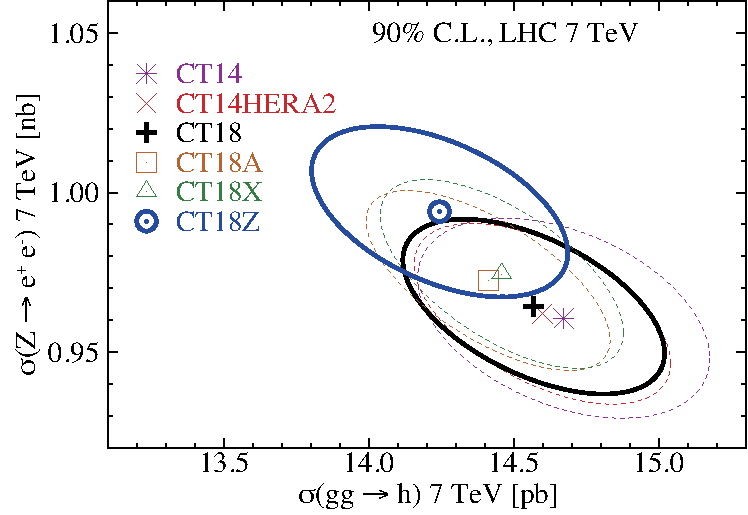
\includegraphics[width=0.44\textwidth]{./fig/sec6/cor_tel_ct18s_H-Z__7TeV_shifted_KP_ect.pdf}
  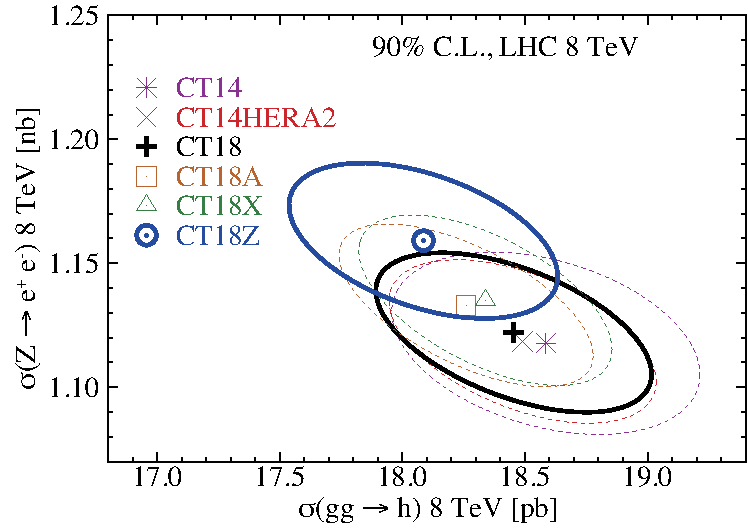
\includegraphics[width=0.44\textwidth]{./fig/sec6/cor_tel_ct18s_H-Z__8TeV_shifted_KP_ect.pdf} \\
  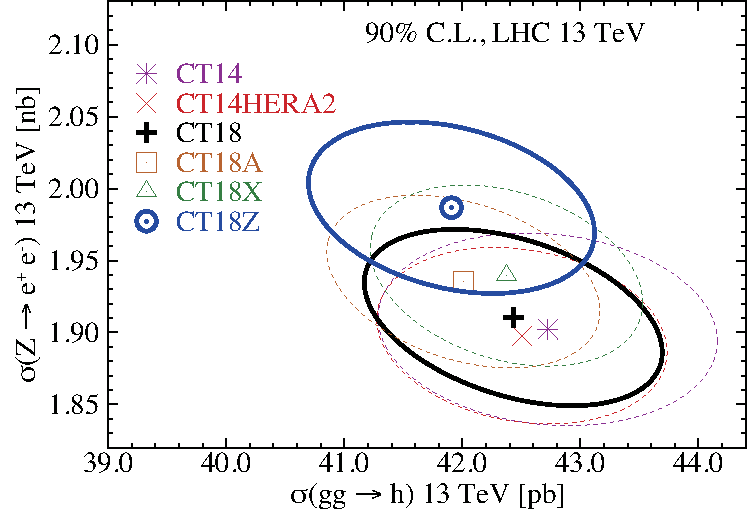
\includegraphics[width=0.44\textwidth]{./fig/sec6/cor_tel_ct18s_H-Z_13TeV_shifted_KP_ect.pdf}
  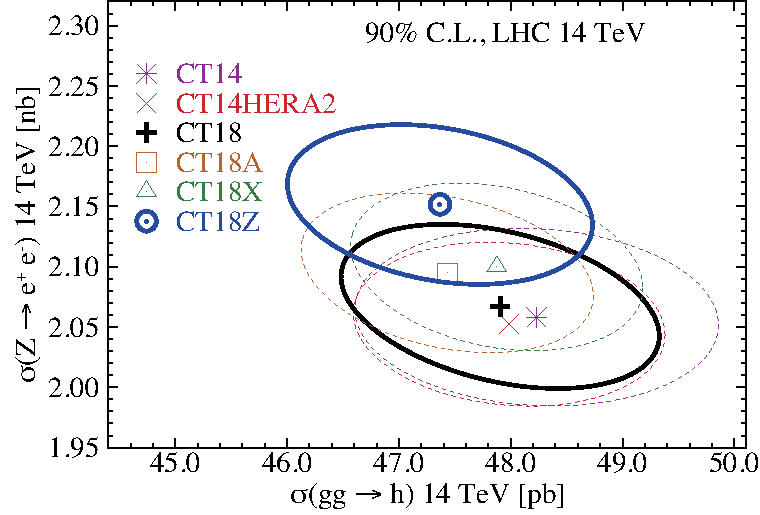
\includegraphics[width=0.44\textwidth]{./fig/sec6/cor_tel_ct18s_H-Z_14TeV_shifted_KP_ect.pdf} \\
  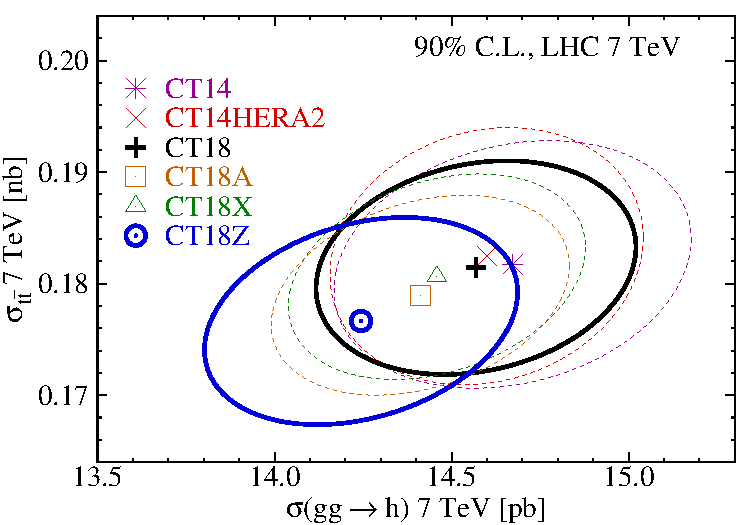
\includegraphics[width=0.44\textwidth]{./fig/sec6/cor_tel_ct18s_H-T__7TeV.pdf}
  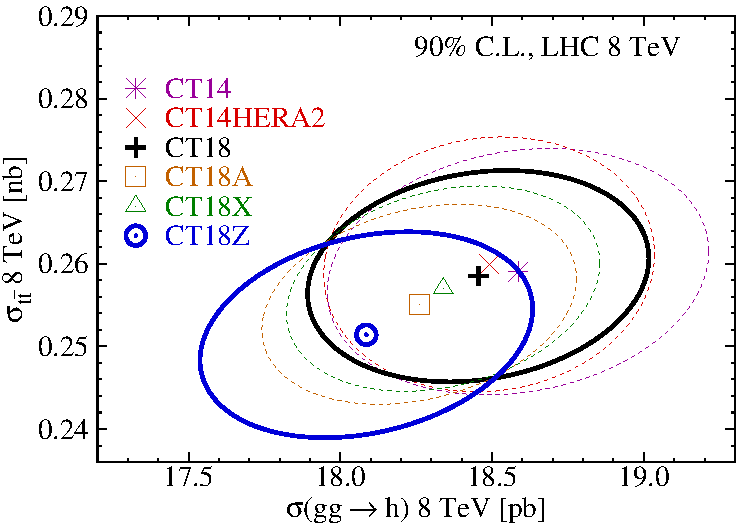
\includegraphics[width=0.44\textwidth]{./fig/sec6/cor_tel_ct18s_H-T__8TeV.pdf} \\
  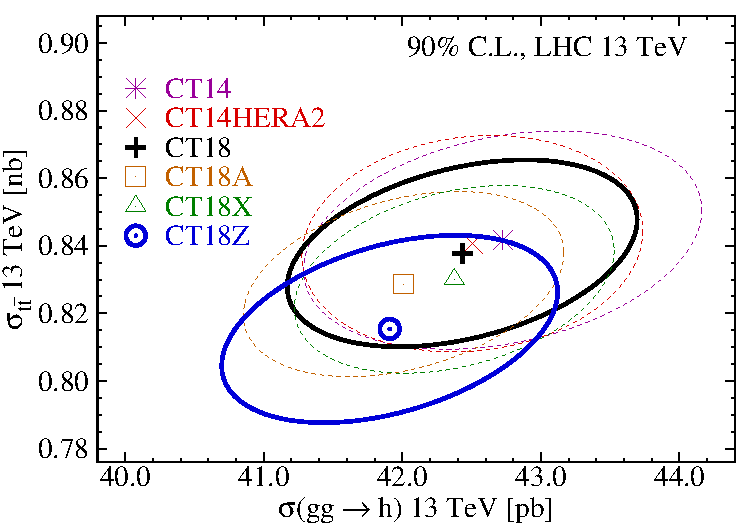
\includegraphics[width=0.44\textwidth]{./fig/sec6/cor_tel_ct18s_H-T_13TeV.pdf}
  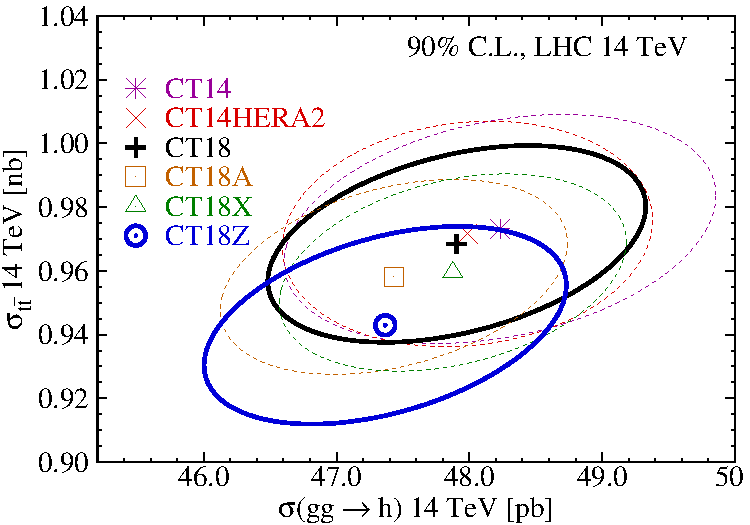
\includegraphics[width=0.44\textwidth]{./fig/sec6/cor_tel_ct18s_H-T_14TeV.pdf} \\
	\end{center}
    \vspace{-2ex}
	\caption{The 90\% C.L. error ellipses for the $ggH$, $t \bar t$, and $Z^0$ inclusive cross sections computed with the CT18 NNLO family of PDFs at the LHC 7, 8, 13 and 14 TeV. 
		\label{fig:corr_ellipse1}}
\end{figure}

\begin{widetext}
\begin{figure}[p]
	\begin{center}
  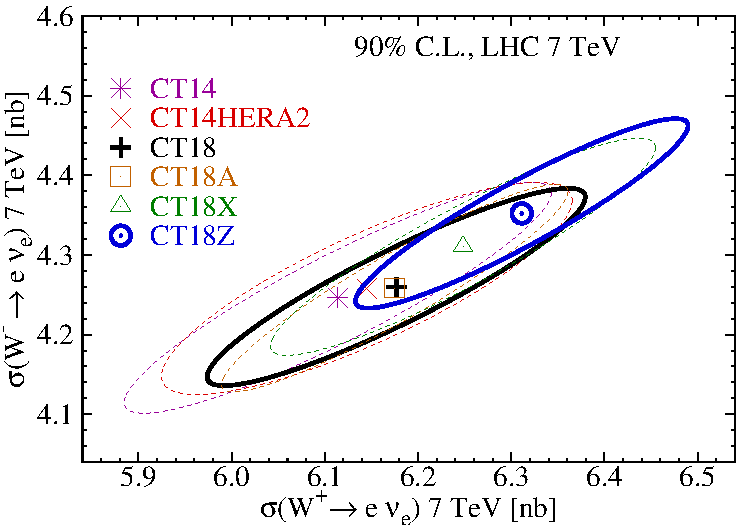
\includegraphics[width=0.44\textwidth]{./fig/sec6/cor_tel_ct18s_Wp-Wm__7TeV_shifted.pdf} 
  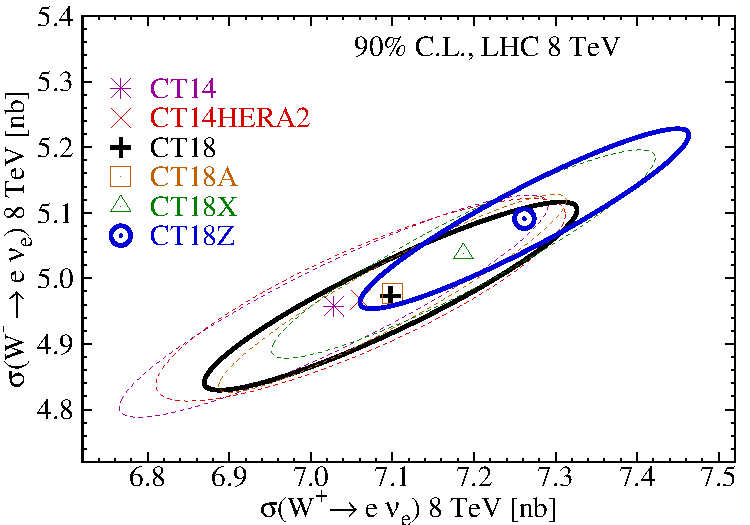
\includegraphics[width=0.44\textwidth]{./fig/sec6/cor_tel_ct18s_Wp-Wm__8TeV_shifted.pdf} \\
  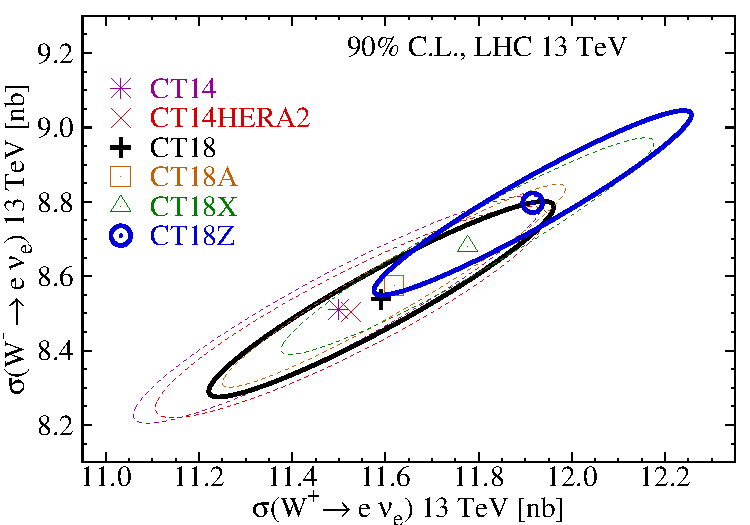
\includegraphics[width=0.44\textwidth]{./fig/sec6/cor_tel_ct18s_Wp-Wm_13TeV_shifted.pdf} 
  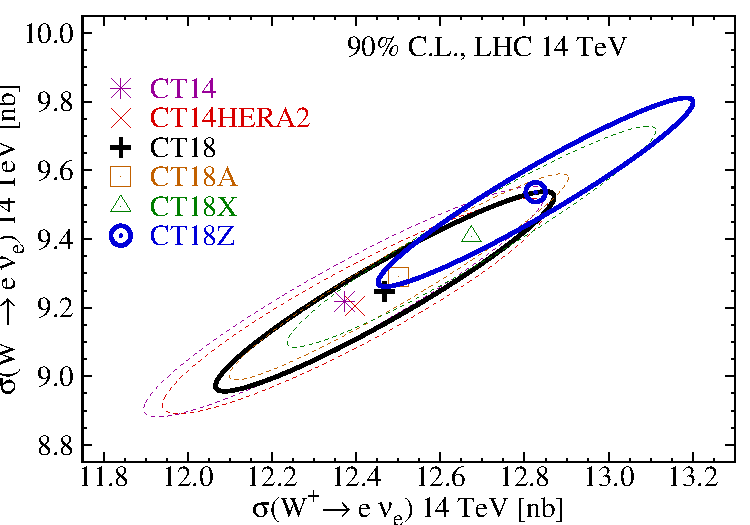
\includegraphics[width=0.44\textwidth]{./fig/sec6/cor_tel_ct18s_Wp-Wm_14TeV_shifted.pdf} \\
  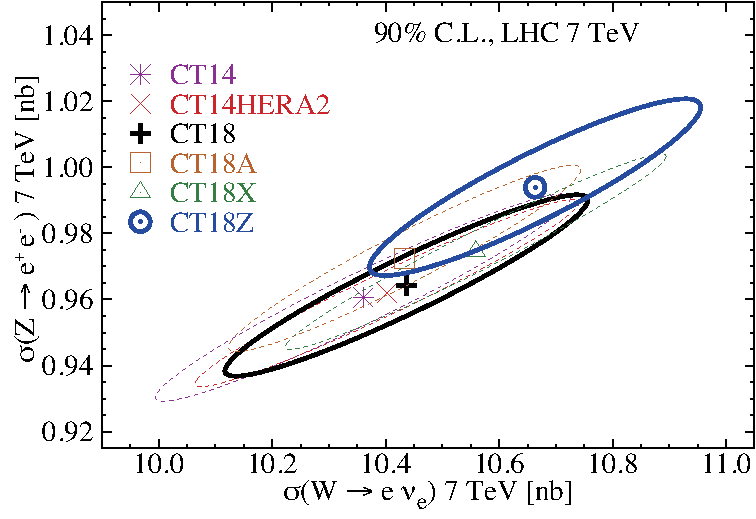
\includegraphics[width=0.44\textwidth]{./fig/sec6/cor_tel_ct18s_W-Z__7TeV_shifted_KP_ect.pdf} 
  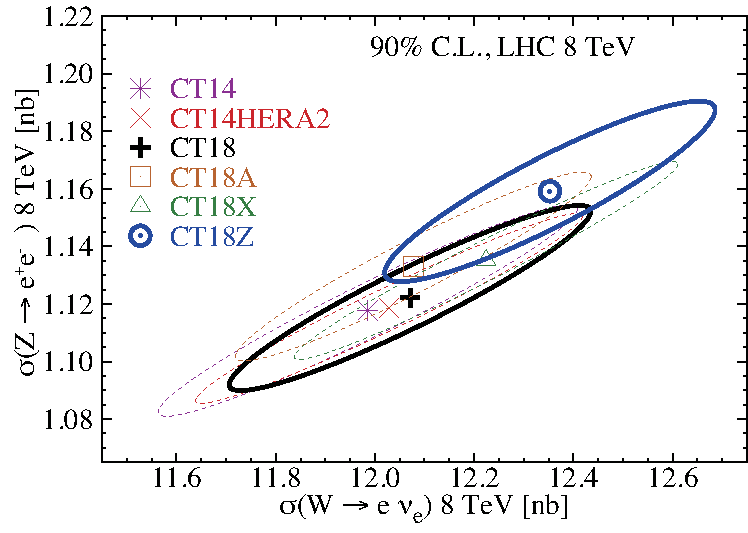
\includegraphics[width=0.44\textwidth]{./fig/sec6/cor_tel_ct18s_W-Z__8TeV_shifted_KP_ect.pdf} \\
  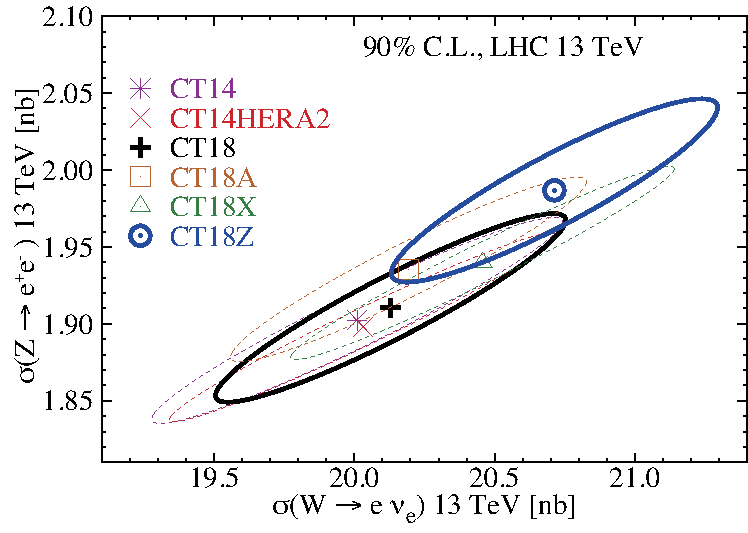
\includegraphics[width=0.44\textwidth]{./fig/sec6/cor_tel_ct18s_W-Z_13TeV_shifted_KP_ect.pdf} 
  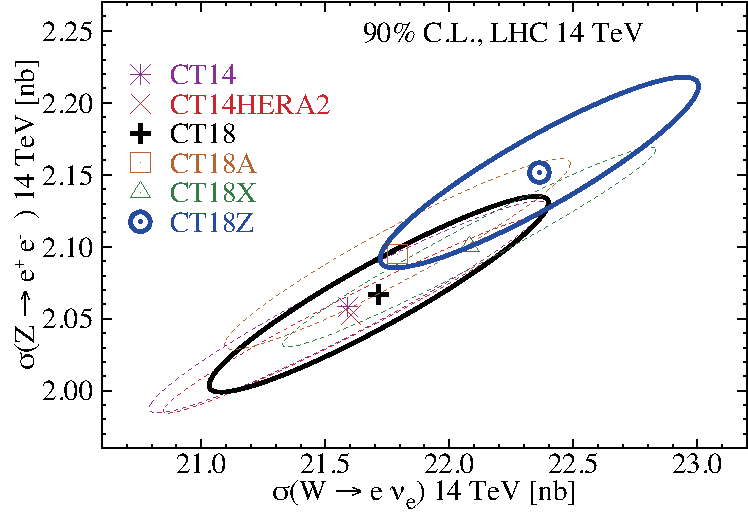
\includegraphics[width=0.44\textwidth]{./fig/sec6/cor_tel_ct18s_W-Z_14TeV_shifted_KP_ect.pdf} \\
	\end{center}
	%    \vspace{-2ex}
	\caption{Same as Fig.~\ref{fig:corr_ellipse1}, but for 
the $W^+$, $W^-$ and $Z^0$ inclusive cross
		sections.
		\label{fig:corr_ellipse2}}
\end{figure}
\end{widetext}

In this work, the masses of the top quark and Higgs boson
are set to $m_t^\mathit{pole}=173.3$ GeV and $m_H=125$ GeV, respectively.
The $W$ and $Z$ inclusive cross sections
(multiplied by branching ratios for the decay into one charged lepton flavor),
are calculated by using the \texttt{Vrap} v0.9 program~\cite{Anastasiou:2003ds,Anastasiou:2003yy} at NNLO in QCD, with the renormalization
and factorization scales ($\mu_R$ and $\mu_F$) set equal
to the invariant mass of the vector boson.
The total inclusive top-quark pair cross sections are calculated with
the help of the program \texttt{Top++}
v2.0~\cite{Czakon:2013goa,Top++} at NNLO+NNLL accuracy, with QCD
scales set to the mass of the top quark \cite{Czakon:2017wor} as is
the default in the \texttt{Top++} framework.
%
The Higgs boson cross sections via gluon-gluon fusion
are calculated at NNLO in QCD by using  the \texttt{iHixs} v1.3
program~\cite{Anastasiou:2011pi},
in the heavy-quark effective theory (HQET) with finite top quark mass correction,
and with the QCD scales set equal
to the Higgs boson mass.

\begin{figure}[tb]
	\begin{center}
		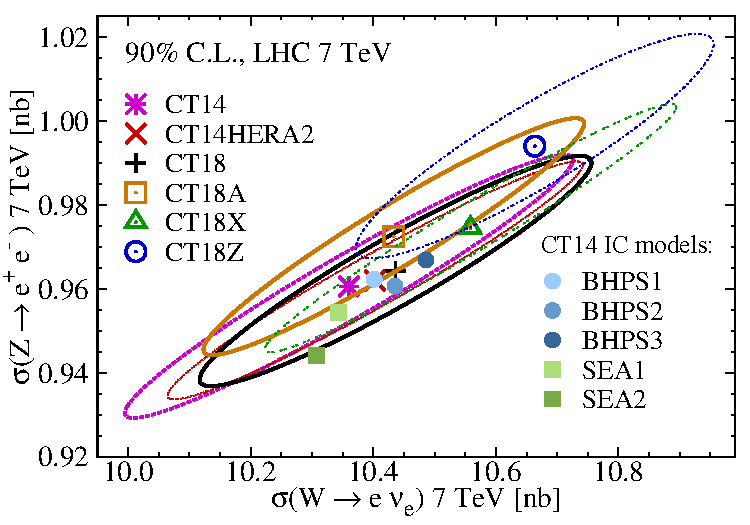
\includegraphics[width=0.65\textwidth]{./fig/sec6/cor_tel_ct18s_W-Z__7TeV_shifted_IC_TH.pdf}
	\end{center}
	\vspace{-2ex}
	\caption{Theoretical predictions of the total production cross sections of $W$ and $Z$ bosons
	at $\sqrt{s}=7$ TeV as relevant for the ATLAS 7 TeV $W/Z$ data (Exp.~ID=248).  Here, we also
	include several calculations which include an intrinsic charm (IC) PDF based upon either
	the BHPS valence-like model (with three different normalizations) or a sea-like model (with
	two different normalizations) in addition to CT14, as described in Ref.~\cite{Hou:2017khm}.
		\label{fig:IC}}
\end{figure}

Fig.~\ref{fig:corr_ellipse1} shows that the Higgs boson cross section through
gluon-gluon fusion ($ggH$) at the LHC does not have a pronounced correlation 
with the top-quark pair ($t \bar t$) cross section, because the two processes are dominated by the gluon
PDF in somewhat different $x$ regions. 
The degree of anti-correlation found in the $ggH$ and $Z$ boson cross sections decreases as the LHC energy increases. 
On the other hand, Fig.~\ref{fig:corr_ellipse2} shows that the electroweak gauge boson cross sections are highly correlated with each other at the LHC.
Generally speaking, the prediction of CT18 is closer to \CTHERAII, and the largest difference occurs between CT18Z and CT14. 
Furthermore, the CT18X prediction is closer to CT18Z for the electroweak gauge boson productions, cf. Fig.~\ref{fig:corr_ellipse2}, but not for the $ggH$ or $t \bar t$ inclusive cross sections, cf. Fig.~\ref{fig:corr_ellipse1}.

The mutual dispositions of the error ellipses for $W$ and $Z$ cross sections in the bottom half of Fig.~\ref{fig:corr_ellipse2} can be tied to the differences among the strangeness and other PDFs of the CT18, A, X, and Z ensembles discussed in Sec.~\ref{sec:CT18ZvsCT18}. In general, the orientations of all shown $W$-$Z$ ellipses are similar, with
the direction parallel to the semi-minor axes --- associated with the relative difference between the $W$ and
$Z$ production cross sections --- most closely identified with the strange PDF. 
The correlation between the $s$-PDF and the ratio of $W^\pm$ to $Z$ cross sections was first pointed out in the CTEQ6.6 analysis~\cite{Nadolsky:2008zw}.
The theory predictions based on
CT18A and CT18Z are both equally shifted in this direction. Meanwhile, CT18X, and especially, CT18Z, are
significantly offset along the semi-major axis [the ``$\sigma(Z)\!+\!\sigma(W)$ direction''], more related to the gluon at $x<10^{-2}$, as again was pointed out in \cite{Nadolsky:2008zw}. 
The close alignment of CT18Z and A in the perpendicular direction relates closely to similarity in the fitted strangeness
distributions obtained under these fits.

It is worthwhile to investigate whether the inclusion of nonperturbative charm may significantly alter these theoretical predictions, especially for electroweak boson production.  In \cite{Ball:2017nwa}, it was suggested that tensions between the combined HERA data (Exp.~ID=160) and
ATLAS 7 TeV $W/Z$ data require that the charm PDF at the initial scale $Q_0$ be independently parameterized.  Such nonperturbative charm, of 
{\it indefinite sign} and shape, was thus implemented using the unique neural network approach of the NNPDF collaboration as a ``fitted charm'' contribution to the proton's structure, distinct from perturbative charm.  The question of intrinsic charm, including the interpretation of its dynamic origin in perturbative QCD, has also been studied by CT, most recently, in Ref.~\cite{Hou:2017khm}, which implemented nonperturbative charm as an explicitly twist-$2$ intrinsic PDF, informed by various models, at the scale $Q_0=m_c$ as a boundary condition for the perturbative evolution of charm.  Following this work, we show in Fig.~\ref{fig:IC} theoretical predictions for the total $W$ and $Z$ production cross sections at 7 TeV, analogous to the third left-hand panel of Fig.~\ref{fig:corr_ellipse2}, but including several scenarios for IC.  In Fig.~\ref{fig:IC}, it can be seen that the inclusion of IC shifts the combined theoretical prediction for the 7 TeV $W$ and $Z$ cross sections along the semi-minor axis in a direction antiparallel to the shift that occurs once the ATLAS 7 TeV data are fitted (CT18 $\to$ CT18A).  The downward shift of the IC predictions in the figure, with respect to the purely extrinsic charm predictions of CT18, etc., appears to be a generic outcome of assuming a {\it non-negative charm} at the initial-scale $Q_0$, which would naturally arise from twist-4 contributions as discussed in \cite{Hou:2017khm}. For this reason, we conclude that inclusion of nonperturbative charm according to the standard approach of including an intrinsic $c_\mathrm{IC}(x,Q=m_c)$ PDF is unlikely to resolve the tensions we describe in detail in Sec.~\ref{sec:AppendixCT18Z}. The subtleties involved in the definition and dynamical origin of intrinsic/fitted charm are sufficiently complex that more forthcoming analyses will be required
to disentangle them and understand their phenomenological implications.


\subsection{Vector boson differential cross sections at the LHC}
\label{sec:Res}

\begin{figure}[htb]
	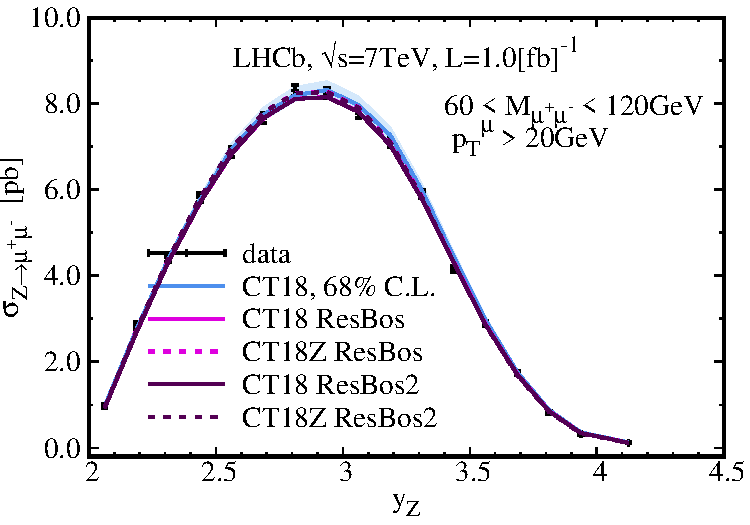
\includegraphics[width=0.49\textwidth]{./fig/sec6/data_245_CT18__1_ect.pdf}
	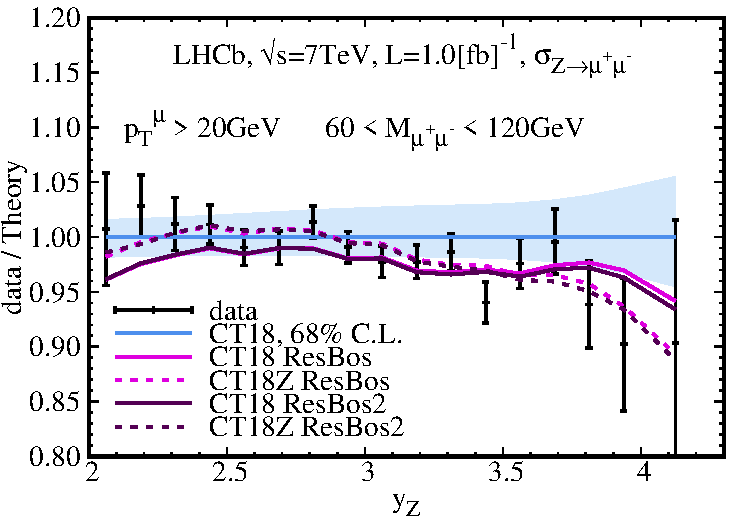
\includegraphics[width=0.49\textwidth]{./fig/sec6/data_245_CT18__1-TcD_ect.pdf}
	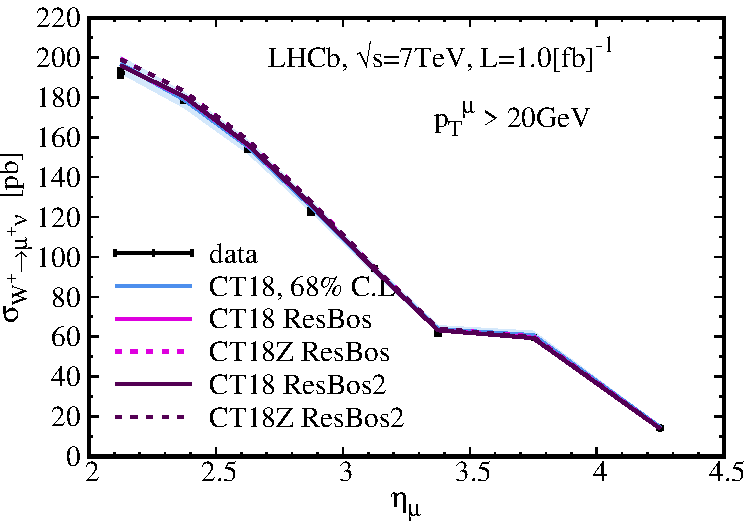
\includegraphics[width=0.49\textwidth]{./fig/sec6/data_245_CT18__2_ect.pdf}
	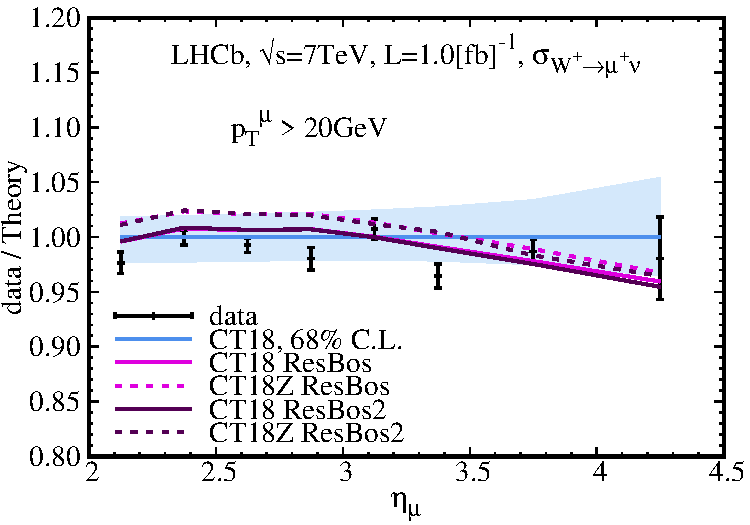
\includegraphics[width=0.49\textwidth]{./fig/sec6/data_245_CT18__2-TcD_ect.pdf}
	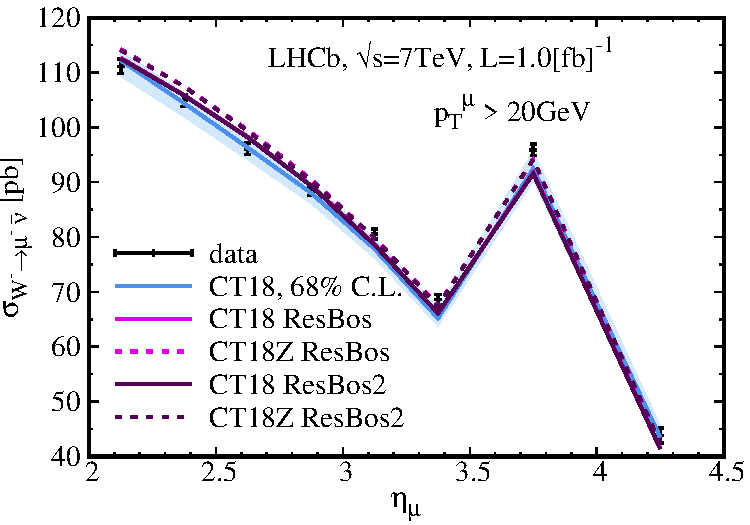
\includegraphics[width=0.49\textwidth]{./fig/sec6/data_245_CT18__3_ect.pdf}
	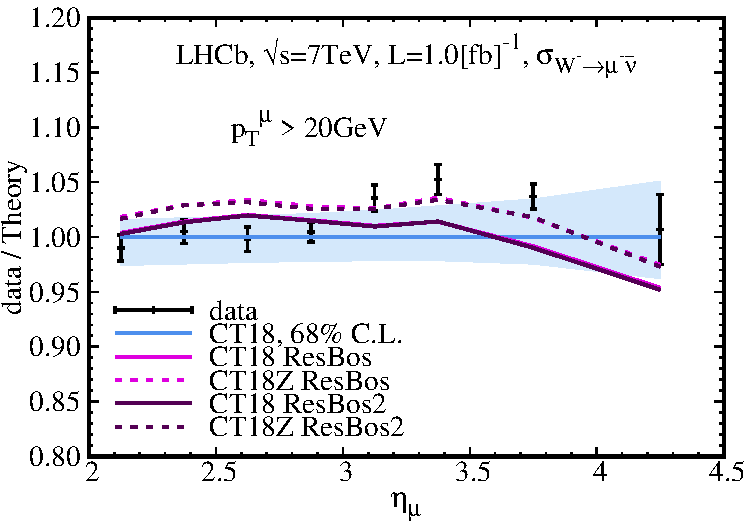
\includegraphics[width=0.49\textwidth]{./fig/sec6/data_245_CT18__3-TcD_ect.pdf}
	\caption{Comparison of the LHCb 7 TeV $W$ and $Z$ data to CT18 predictions, with either NNLO (labeled by CT18) or ResBos (labeled by CT18 ResBos) calculations. The prediction of CT18Z with ResBos calculation (CT18Z ResBos) is also shown for comparison.  
		\label{fig:245_res}}
\end{figure}

As described previously, NNLO calculations have been used formerly to predict vector boson production data at both the Tevatron and LHC. 
In the past, we have also compared this type of precision data to ResBos predictions, which include effects from multi-gluon emission \cite{Balazs:1997xd}, to produce the CTEQ6.6, CT10 and CT14 PDFs.  
For this reason, it is important to compare vector boson differential cross section measurements to predictions based on the CT18 (and CT18Z) PDFs with ResBos and NNLO calculations.
As an example, we compare the ResBos predictions to the LHCb 7 TeV $W$ and $Z$ boson differential distributions~\cite{Aaij:2015gna} in Fig.~\ref{fig:245_res}. 

For completeness, we have also included in the same figure the predictions from ResBos2, which is an updated version of the ResBos project to include full NNLO corrections, {\it i.e.}, the complete $\alpha_s^2$ contribution for Drell-Yan production of the dilepton pair has been included in this calculation \cite{resbos2-paper}. 
In contrast, the ResBos prediction only contains parts of the NNLO contribution. More specifically, it includes only the Wilson coefficient $C^{(1)}$, but not $C^{(2)}$, in the resummation calculation, cf.~Ref.~\cite{Balazs:1997xd}. 
As shown in Fig.~\ref{fig:245_res}, the predictions from ResBos and ResBos2 agree well for the LHCb kinematics, except in the very large rapidity region. 
The difference between the resummed and (NNLO) fixed-order predictions arises from multiple soft-gluon radiation, the effect of which tends to grow in the large-rapidity
region, where it becomes comparable in size to the LHCb 7 TeV experimental errors. Further detailed discussion about the difference between the resummation and fixed-order calculations will be presented elsewhere. 
In order to see how different PDFs might modify these comparisons between theory predictions and the LHCb 7 TeV data, we also present in the same plot predictions based upon the CT18Z PDFs, in which the gluon and sea quark distributions differ from those of CT18.

\subsection{$W$ plus charm-jet production at the LHC}
\label{sec:Wcharm}

\begin{figure}[tb]
	\begin{center}
		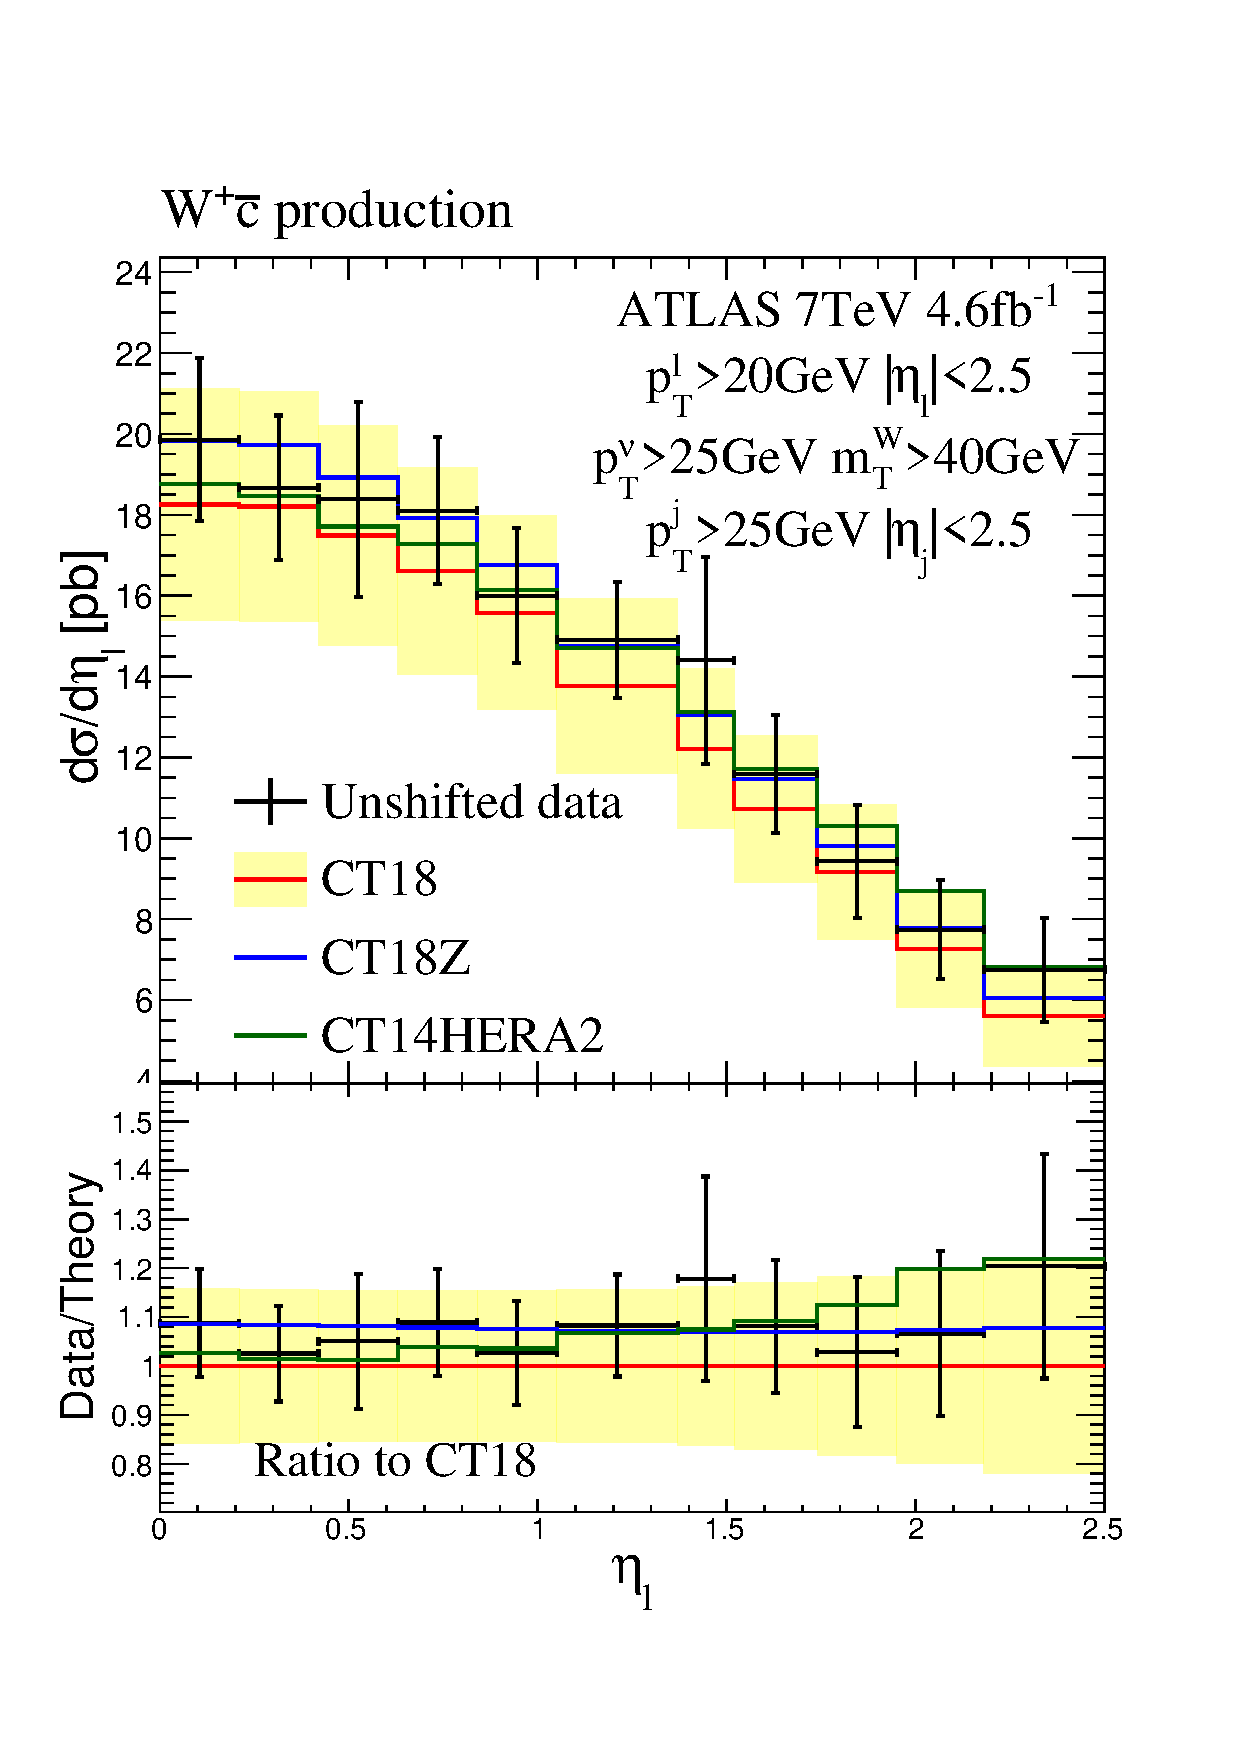
\includegraphics[width=0.45\textwidth]{./fig/sec6/hepdata_mcfm_grid-WpCbar-ATLAS7_etal_CT18NNLO_mcfm_grid-WpCbar-ATLAS7_etal_CT18ZNNLO_mcfm_grid-WmCjet-ATLAS7_etal_CT14HERA2NNLO.pdf}
		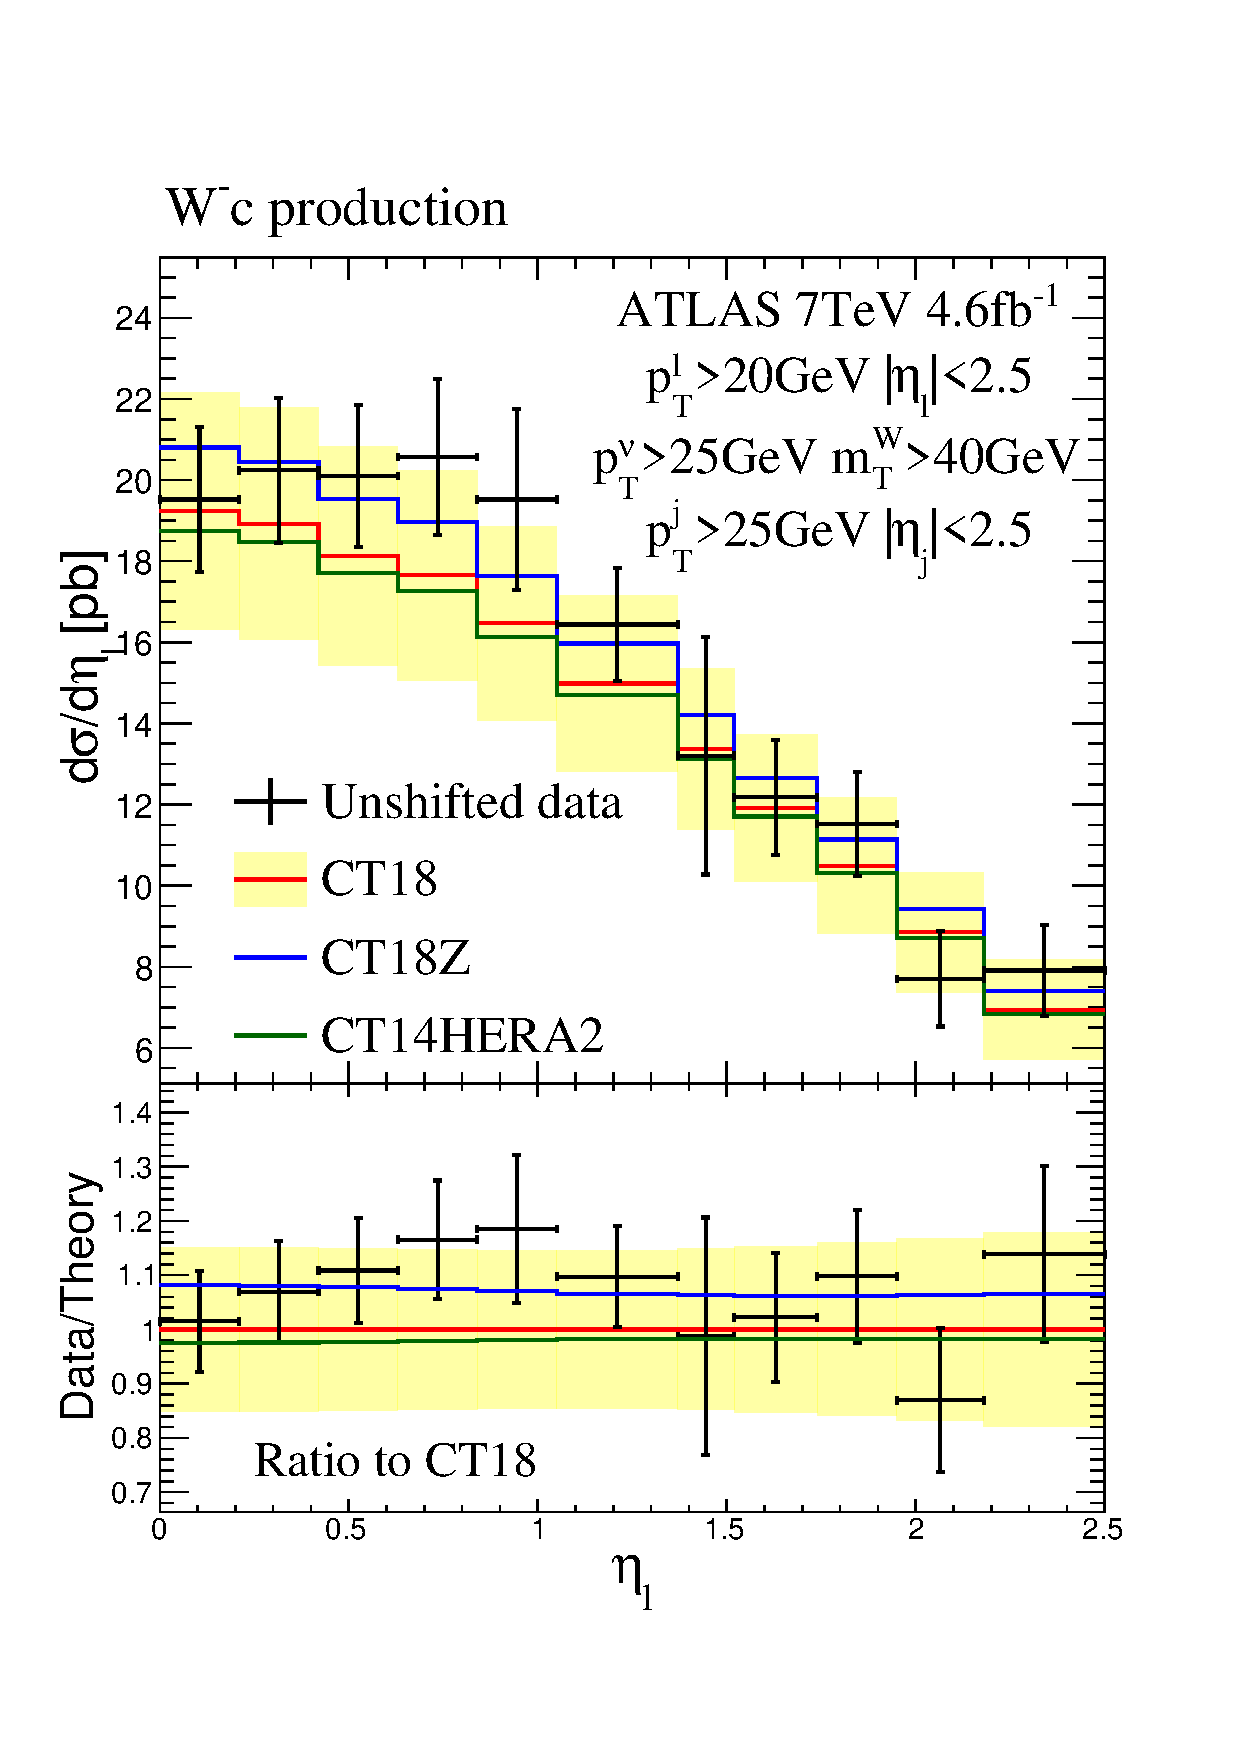
\includegraphics[width=0.45\textwidth]{./fig/sec6/hepdata_mcfm_grid-WmCjet-ATLAS7_etal_CT18NNLO_mcfm_grid-WmCjet-ATLAS7_etal_CT18ZNNLO_mcfm_grid-WmCjet-ATLAS7_etal_CT14HERA2NNLO.pdf}
	\end{center}
	\vspace{-2ex}
	\caption{Comparison of the CT18(Z) and \CTHERAII~NNLO predictions for ATLAS 7 TeV $W^+ + \bar{c}$-jet (left) 
		and $W^-\! +\! c$-jet (right) production, respectively.
		\label{fig:atl7wpcbar}}
\end{figure}

The $s$-quark PDF of CT18 differs from CT14 at $x < 10^{-1}$ predominantly as a result of the inclusion of the new LHC vector boson production data from  LHCb and ATLAS 7 TeV. Independent constraints on 
the strange quark are provided by the cross sections with significant contributions of  processes initiated by $s$ quarks, such as $W$ plus charm-jet production~\cite{Yalkun:2019gah}. As this process has not yet been calculated to NNLO, the relevant data samples have not been included in the CT18(Z) NNLO PDF fit, but it is still instructive to compare the NLO predictions (but with the NNLO PDFs) with the data. 

Fig.~\ref{fig:atl7wpcbar} compares the \CTHERAII, CT18 and CT18Z predictions with ATLAS 7 TeV $W^+ + \bar{c}$-jet and $W^-\! +\! c$-jet data, respectively. The theoretical calculations are performed by using \texttt{APPLgrid} tables generated with \texttt{MCFM}, cross checked against \texttt{MadGraph\_aMC@NLO}+\texttt{aMCfast}. The $\chi^2/N_{pt}$ values are 0.59, 0.52 and 0.41, respectively, with the \CTHERAII, CT18 and CT18Z PDFs, for the total of $N_{pt}=22$ data points.
We observe an upward shift in the predictions based upon CT18Z compared with CT18 in both panels of Fig.~\ref{fig:atl7wpcbar} for $W^+$ and $W^-$. 

Interestingly, for $W^+\bar{c}$ production, the 
\CTHERAII~predictions tend to be even larger than those of CT18(Z) in the large-rapidity region, while for $W^-c$ production in the
right panel of Fig.~\ref{fig:atl7wpcbar}, the \CTHERAII~predictions lie well below the CT18(Z) predictions over the full plotted range. This 
nuanced behavior of the large-rapidity $W^+c$ cross section reflects not only the increase of $s$-quark PDFs in CT18Z, but also some compensating changes in $g$, $d$ and other PDFs that occur at large $x$ and have been independently verified by updating the \CTHERAII\, PDFs using $W+c$ cross sections with the \texttt{ePump} program.

%
\begin{figure}[tb]
\begin{center}
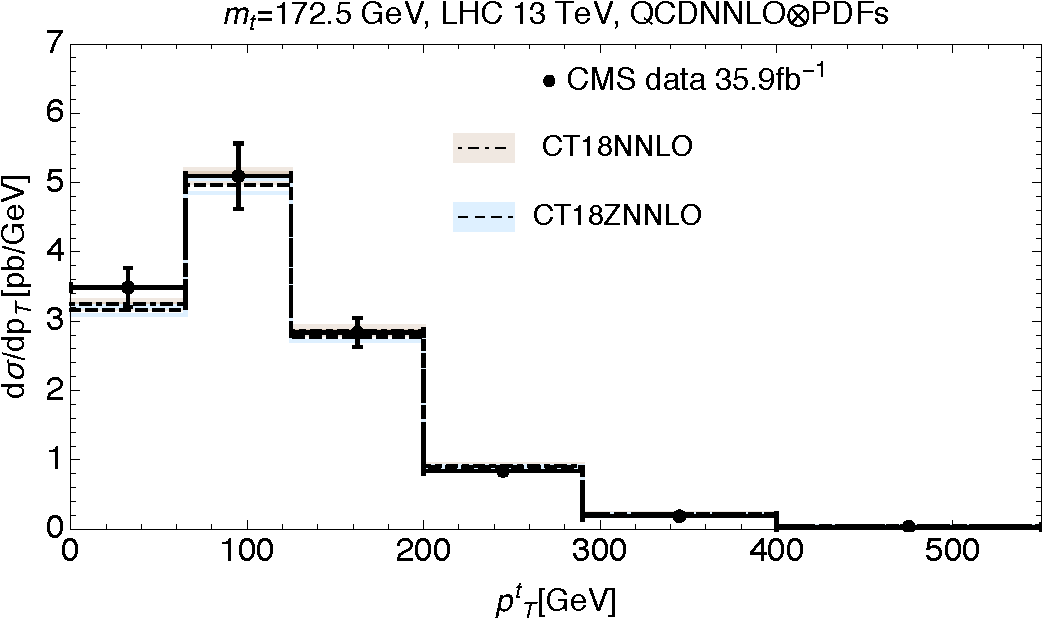
\includegraphics[width=8cm]{./fig/ttbar/CMS13-pT-top-CT18NNLO-mt172p5_ect.pdf}
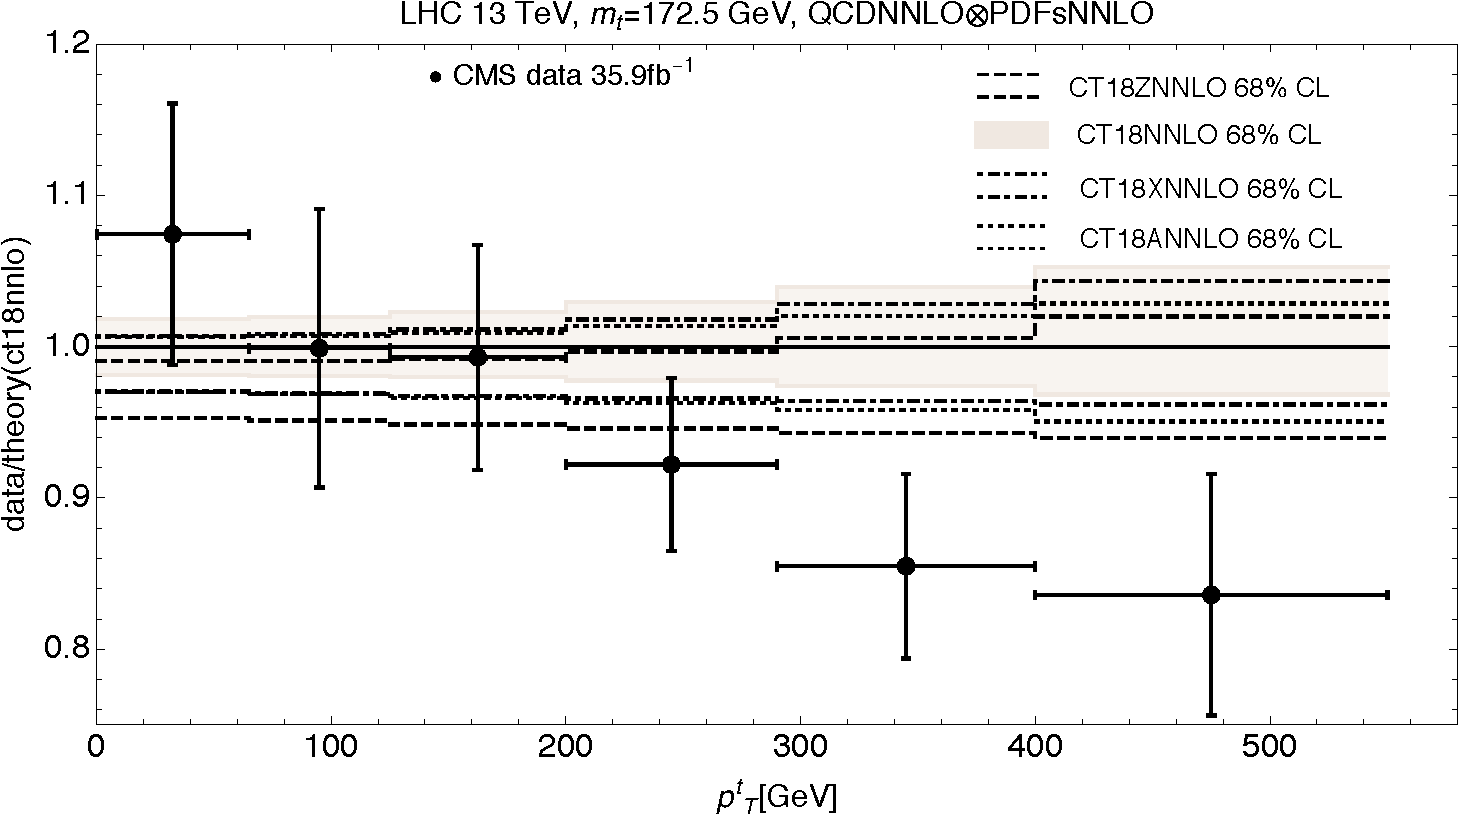
\includegraphics[width=8cm]{./fig/ttbar/CMS13-pt-top-nnlo-ct18-zaxnnlo-mt172p5_ect.pdf}
\caption{Left: Top-quark transverse momentum $p_{T,t}$ distribution. 
Right: data vs theory plot including CT18Z, CT18X, CT18A NNLO. All theory predictions are normalized to the default PDF choice CT18NNLO.
The uncertainties in the data points are statistical and systematic errors summed in quadrature.}
\label{pTt}
\end{center}
\end{figure}

\subsection{Top quark pair differential distributions at the LHC 13 TeV}
\label{sec:tt13}

In Sec.~\ref{sec:QualityTopData}, we have shown data-to-theory comparisons to the ATLAS and CMS differential top-production data at 8 TeV, i.e., data which were included in the CT18(Z) fits. In this section we present analogous comparisons for the CMS 13 TeV measurement of $t\bar t$ differential cross 
sections in the dilepton channel \cite{Sirunyan:2018ucr}. These data have been released after the CT18(Z) data sets were frozen in the final form. The QCD theoretical predictions at NNLO in QCD are obtained by using \texttt{fastNNLO} tables~\cite{fastnnlo:grids} with CT18 NNLO PDFs. The value of the top-quark mass used to obtain the theory predictions in this case is $m_t^{\rm pole}=172.5$ GeV.
We also show the resultant theory predictions using CT18Z, CT18X, and CT18A NNLO PDFs,
with PDF uncertainties for the cross sections shown at the 68\% C.L.
Plots of the distributions and data-vs-theory comparisons are shown in Figs.~\ref{pTt}-\ref{Mtt}. 
In the data-vs-theory plots, all theory predictions are normalized to the default PDF choice, CT18 NNLO. 
The uncertainties in the data points are computed by summing statistical and systematic errors in quadrature.
We observe a clear difference in the slope between the theory and unshifted experimental data for both $d\sigma / dp^t_T$ and $d\sigma / dm_{t\bar{t}}$.
Those differences can be accommodated by systematic error shifts of the data, resulting in a good $\chi^2$ after all uncertainties are taken into account.
We notice that, in the case of the $p_T$ spectrum, the theory prediction obtained with CT18Z NNLO gives a slightly better description of the data at large $p_T$.


%
%\begin{figure}
%\begin{center}
%\includegraphics[width=8.3cm]{./fig/ttbar/CMS13-pTttb-CT18 NNLO-mt172p5.pdf}
%\includegraphics[width=8.3cm]{./fig/ttbar/CMS13-pTtt-nnlo-ct18-zaxnnlo-mt172p5.pdf}
%\caption{Left: transverse momentum $p_{T,tt}$ spectrum of the $t\bar{t}$ pair.
%Right: data vs theory plot including CT18, CT18Z, CT18X, CT18A NNLO. All theory predictions are normalized to the default PDF choice CT18NNLO.}
%\label{pTtt}
%\end{center}
%\end{figure}


\begin{figure}[tb]
\begin{center}
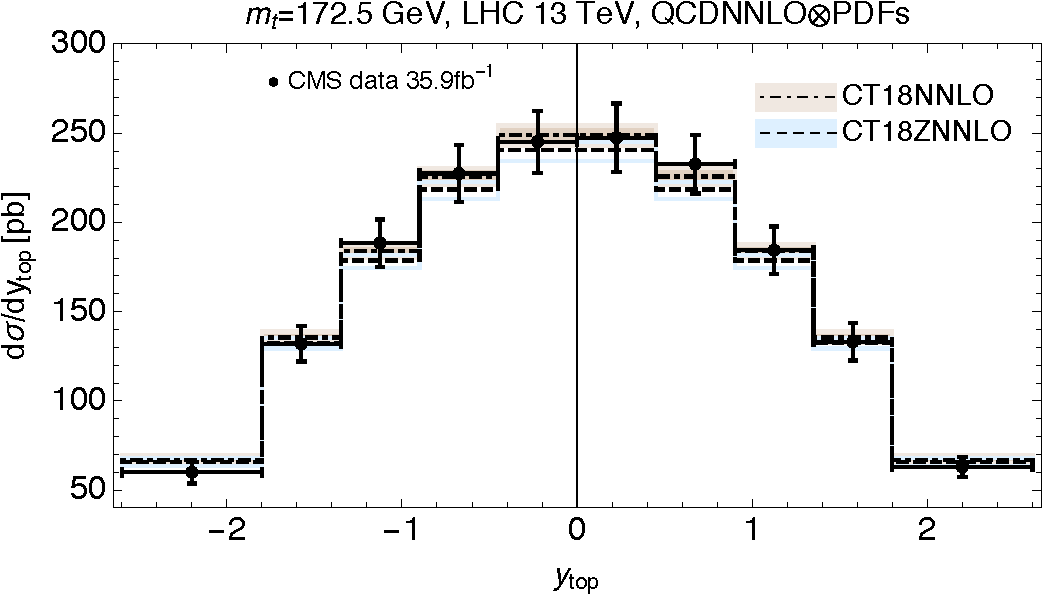
\includegraphics[width=8cm]{./fig/ttbar/CMS13-y-top-CT18NNLO-mt172p5_ect.pdf}
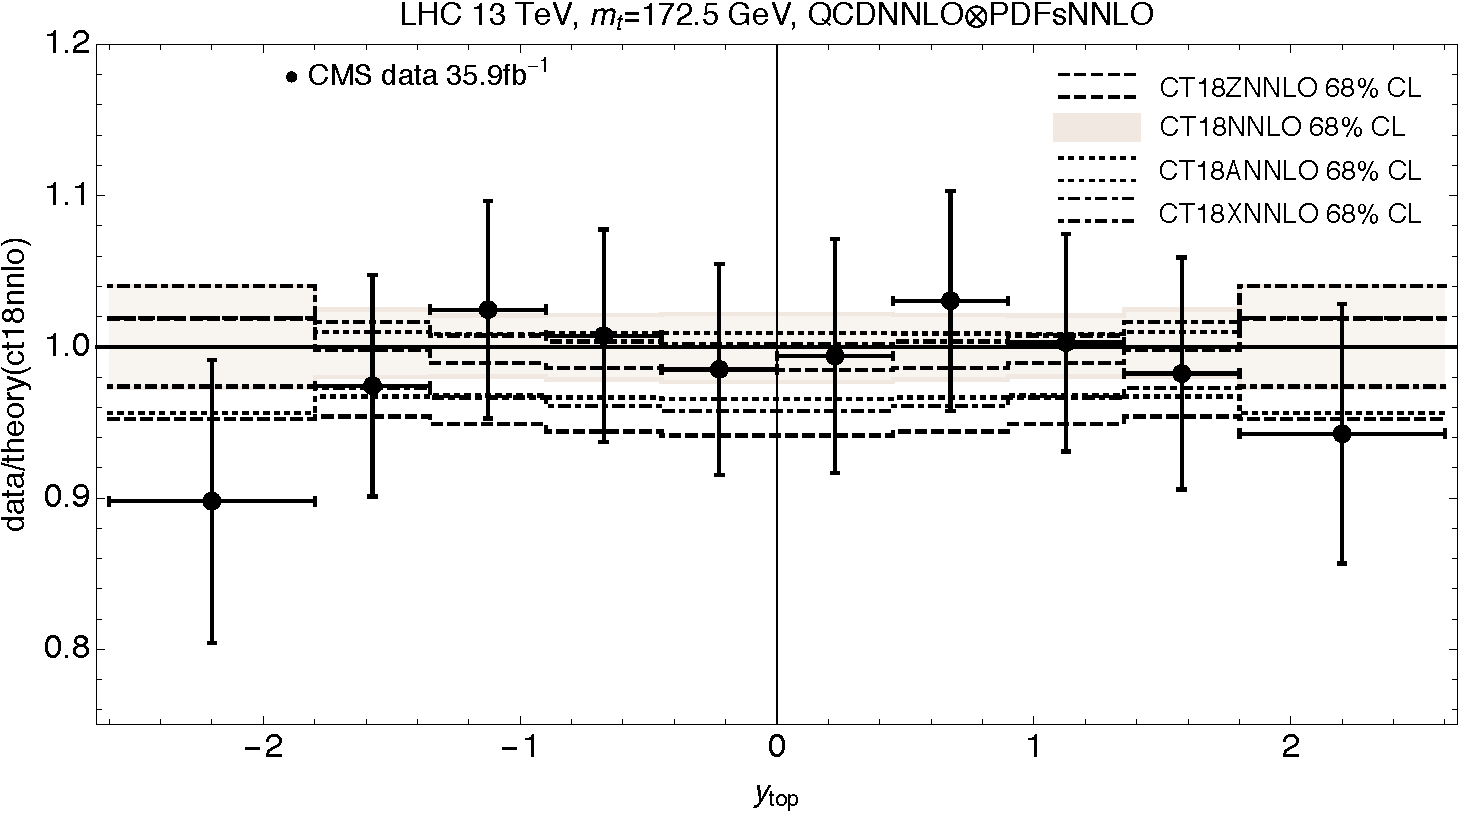
\includegraphics[width=8cm]{./fig/ttbar/CMS13-y-top-nnlo-ct18-zaxnnlo-mt172p5_ect.pdf}
\caption{Left: Top-quark rapidity $y^t$ distribution. 
Right: data vs theory plot including CT18, CT18Z, CT18X, CT18A NNLO. All theory predictions are normalized to the default PDF choice CT18 NNLO.
The uncertainties in the data points are statistical and systematic errors summed in quadrature.}
\label{yt}
\end{center}
\end{figure}


%\begin{figure}
%\begin{center}
%\includegraphics[width=8.3cm]{./fig/ttbar/CMS13-ytt-CT18NNLO-mt172p5.pdf}
%\includegraphics[width=8.3cm]{./fig/ttbar/CMS13-ytt-nnlo-ct18-zxannlo-mt172p5.pdf}
%\caption{Left: rapidity $y^{tt}$ spectrum of the $t\bar{t}$ pair. 
%Right: data vs theory plot including CT18, CT18Z, CT18X, CT18A NNLO. All theory predictions are normalized to the default PDF choice CT18NNLO.}
%\label{ytt}
%\end{center}
%\end{figure}


\begin{figure}[p]
\begin{center}
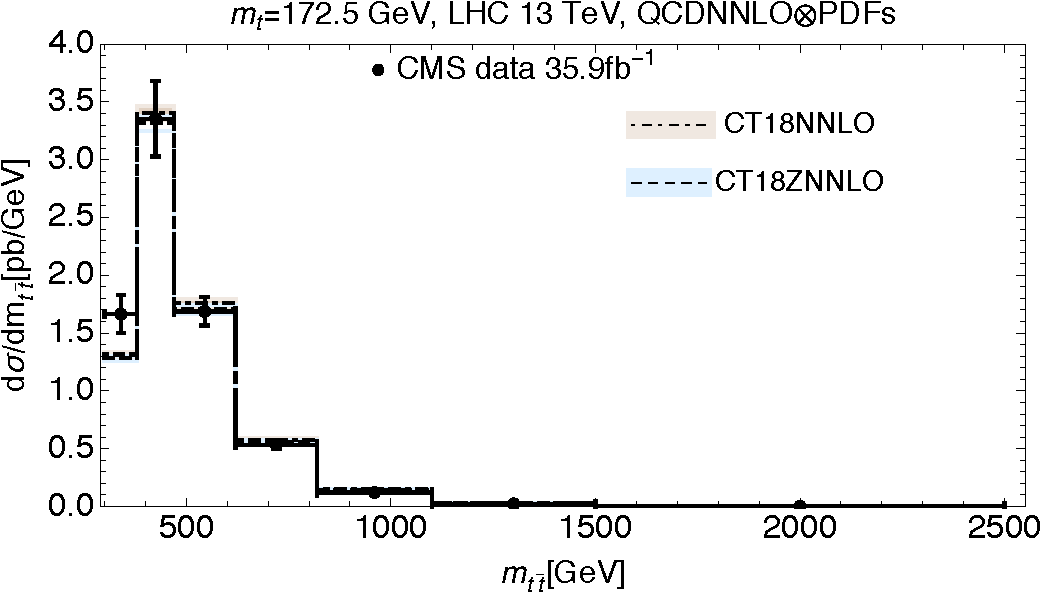
\includegraphics[width=8cm]{./fig/ttbar/CMS13-mtt-CT18NNLO-mt172p5_ect.pdf}
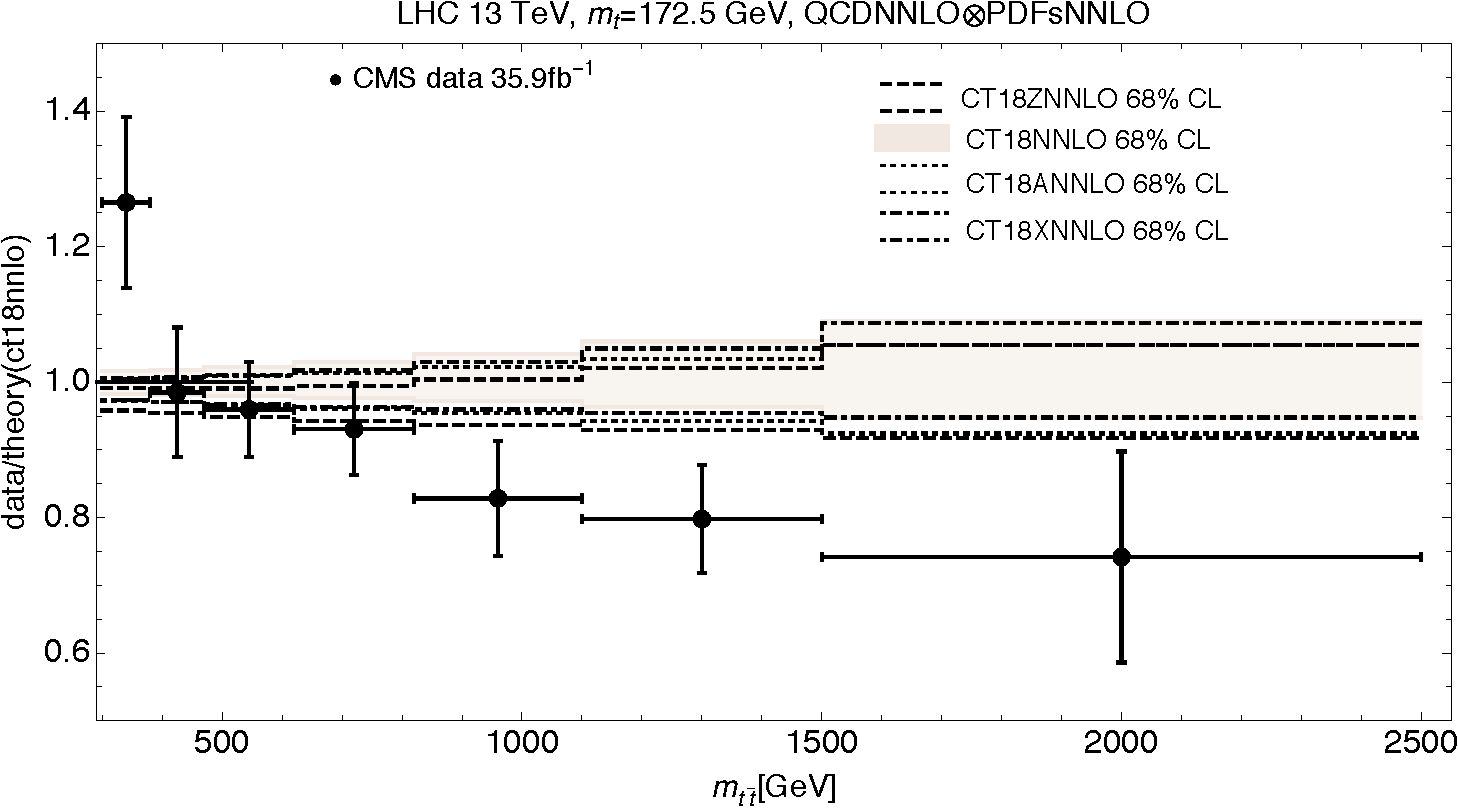
\includegraphics[width=8cm]{./fig/ttbar/CMS13-mtt-top-nnlo-ct18-zaxnnlo-mt172p5_ect.pdf}
\caption{Left: invariant mass distribution of the top-quark pair. 
Right: data vs theory plot including CT18, CT18Z, CT18X, CT18A NNLO. All theory predictions are normalized to the default PDF choice CT18 NNLO.
The uncertainties in the data points are statistical and systematic errors summed in quadrature.}
\label{Mtt}
\end{center}
\end{figure}

%
The impact of the electroweak corrections on the CT18 theory is illustrated in Fig.~\ref{MttEW}. These corrections are included as $K$-factors using the multiplicative scheme according to Ref.~\cite{Czakon:2017wor}. They are available at~\cite{EW:kfac}. Large EW effects show up in the high $p_{T}^t$ tails. 
However, in the $p_T$ range 1 - 500 GeV shown in the figures, 
the EW corrections are not larger than 3-4\% in most cases. 
If one considers higher-$p_T$ regions, $K$-factors would be much larger there.
The EW corrections minimally improve the agreement of theory and data for the
top-quark $p_T$ and $m_{t\bar{t}}$ distributions. 
The $\chi^2/N_{pt}$ of the NNLO QCD $+$ NLO EW prediction using CT18 PDFs agrees well with the values presented in Table 49 of Ref.~\cite{Sirunyan:2018ucr}. 
For all other distributions, the EW corrections are negligible for the kinematic ranges studied.
The CT18 global analysis currently includes $\bar{t}t$ differential cross section measurements from ATLAS and CMS at 8 TeV only. The CT18 theory prediction for these distributions in the fit does not include EW corrections. If EW corrections were included in the fit their impact on the fitted PDFs would be negligible due to the size of the EW corrections in the kinematic range of the distributions currently considered. 

%
%In our CT18 analysis, we have included the 8 TeV $t \bar t$ double differential distribution data from both CMS and ATLAS, as described in previous sections. 
%Before closing this section, we would like to comment on the comparison of CT18 PDF prediction to the recent CMS 13 TeV $t \bar t$ differential cross section measurement at the LHC.

\begin{figure}
\begin{center}
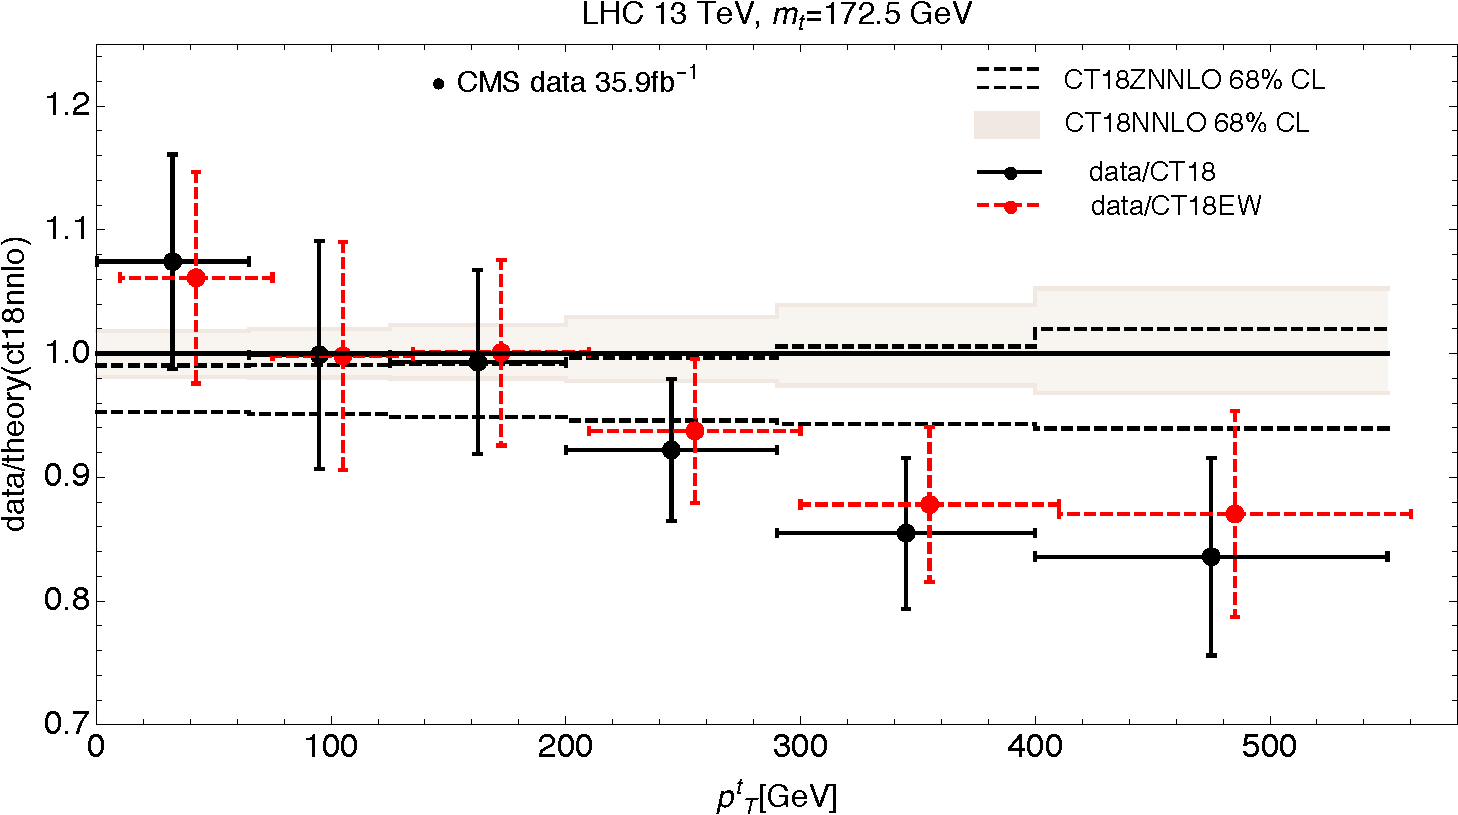
\includegraphics[width=8cm]{./fig/ttbar/CMS13-pt-top-qcdnnloewnlo-ct18nnlo-mt172p5_ect.pdf}
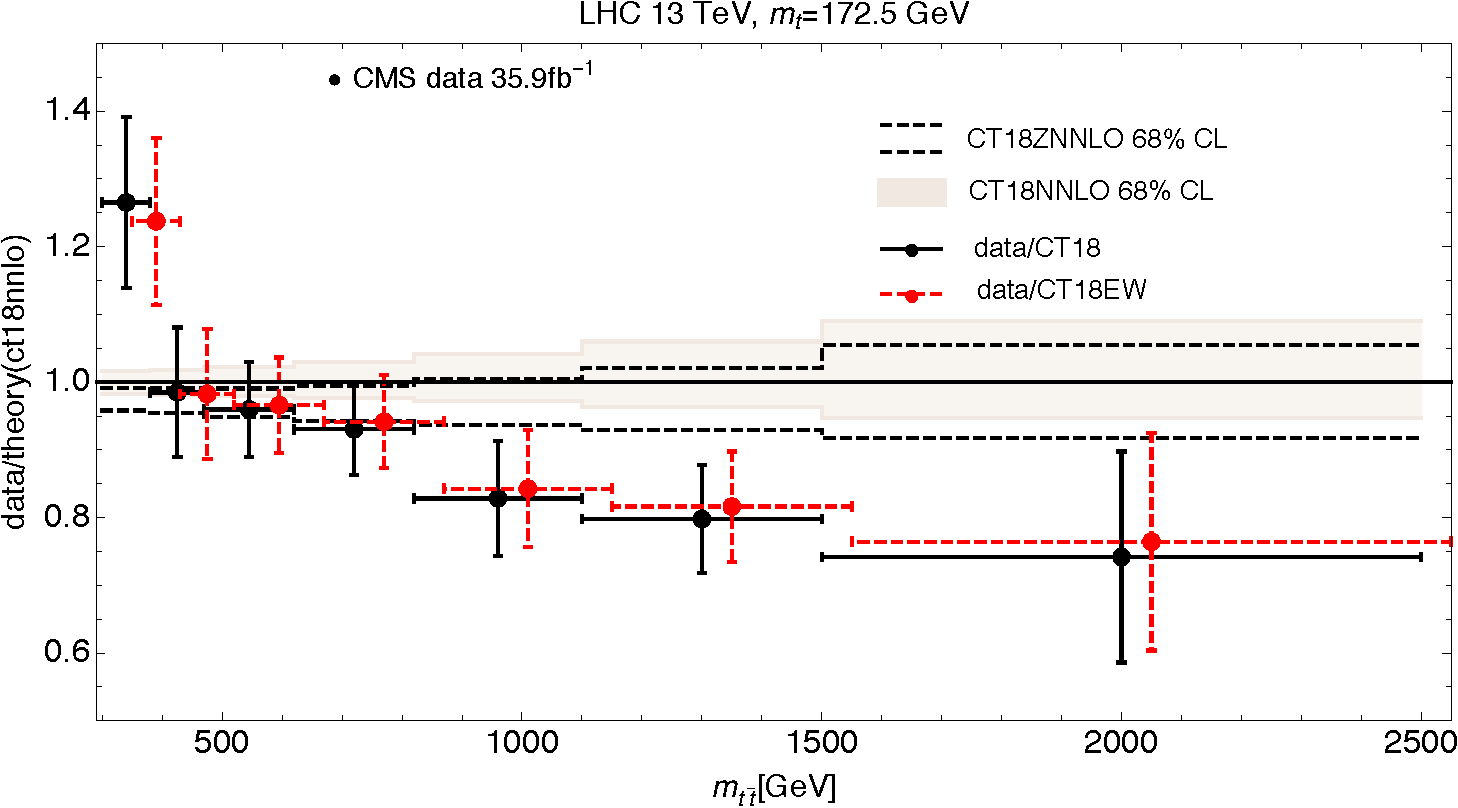
\includegraphics[width=8cm]{./fig/ttbar/CMS13-mtt-qcdnnloewnlo-ct18nnlo-mt172p5_ect.pdf}
\caption{Impact of NLO EW corrections. Data vs theory plot for top-quark $p_T$ distribution and the invariant mass distribution of the $t\bar{t}$ pair. 
The uncertainties in the data points are statistical and systematic errors summed in quadrature. The red data points with dashed error bars represent data divided by the CT18NNLO theory with NLO EW corrections. The black data points with solid error bars represent data normalized to the CT18NNLO theory. The CT18ZNNLO theory prediction (black dashed error band) is also normalized to CT18NNLO. The data vs (theory+EW) points are slightly shifted to the right in the same bin to improve visualization.}
\label{MttEW}
\end{center}
\end{figure}
%

\begin{figure}[h]
%	\includegraphics[width=0.49\textwidth]{./fig/sec6/pdfs_i2Tn3_i2Tn3pCMS13Attmtt_ET1_i2Tn3pCMS13Attmtt_ET2_100GeV_A90CL__00___glu__pdf2_cus-lin.pdf}
%	\includegraphics[width=0.49\textwidth]{./fig/sec6/pdfs_i2Tn3_i2Tn3pCMS13Attmtt_ET1_i2Tn3pCMS13Attmtt_ET2_100GeV_A90CL__00___glu__pdfr_cus-lin.pdf}
%	\includegraphics[width=0.49\textwidth]{./fig/sec6/pdfs_i2Tn3_i2Tn3pCMS13Attmtt_ET1_i2Tn3pCMS13Attmtt_ET2_100GeV_A90CL__00___glu_xpdf__cus-lin.pdf}
	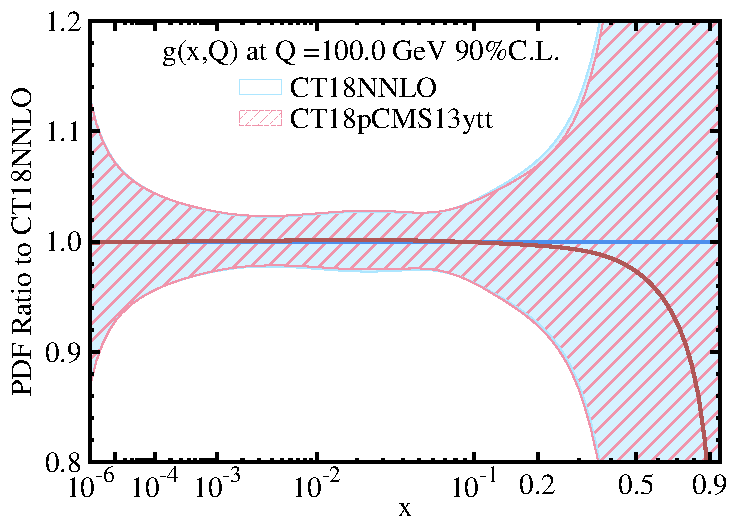
\includegraphics[width=0.49\textwidth]{./fig/sec6/pdfs_CT18NNLO-58_CT18pCMS13ytt_100-0GeV_S90CL__00___glu__pdfr_cus-lin.pdf}
	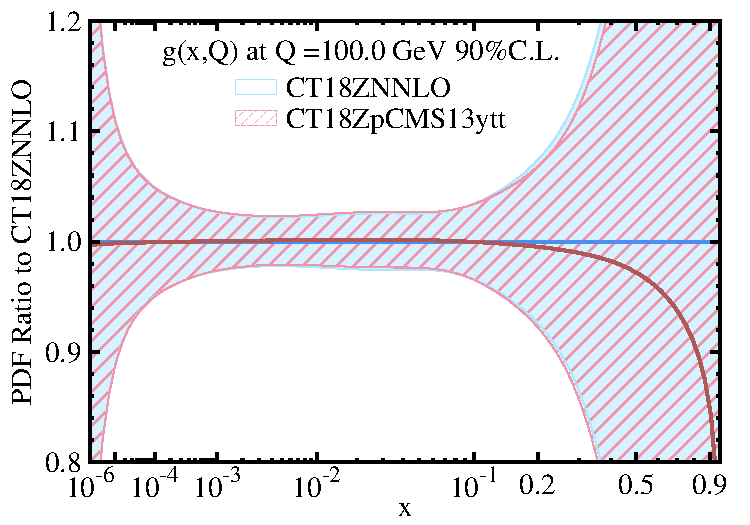
\includegraphics[width=0.49\textwidth]{./fig/sec6/pdfs_CT18ZNNLO-58_CT18ZpCMS13ytt_100-0GeV_S90CL__00___glu__pdfr_cus-lin.pdf}
	\caption{Impact of the $y_{t \bar t}$ differential cross section measurements of the CMS 13 TeV $t \bar t$ data on the CT18 (left) and CT18Z (right) gluon PDFs. 
	\label{fig:cms13ytt}}
\end{figure}

%
Among various one-dimensional $t \bar{t}$ differential distributions, the distribution of the top-quark pair rapidity, $y_{t \bar t}$, shows a good agreement between the CMS data and CT18 predictions. 
To examine how this data could modify the CT18(Z) gluon PDFs, we use the \texttt{ePump} program~\cite{Hou:2019gfw} to update the CT18(Z) PDFs, after including the CMS 13 TeV $y_{t \bar t}$ data in the fit. 
As shown in Fig.~\ref{fig:cms13ytt}, the updated gluon-PDF error band (labeled as CT18pCMS13ytt) is very slightly reduced for $x$ from 0.1 to 0.4 in both cases.
Further discussion about these data sets will be presented elsewhere. 

%\begin{figure}[!htb]
%\begin{center}
%\includegraphics[width=8.3cm]{./fig/ttbar/CMS13-pt-top-qcdnnloewnlo-ct18nnlo-mt172p5.pdf}
%\includegraphics[width=8.3cm]{./fig/ttbar/CMS13-ptt-qcdnnloewnlo-ct18nnlo-mt172p5.pdf}
%\caption{Impact of NLO EW corrections. Left: data vs theory plot for top-quark $p_T$ distribution. 
%Right: data vs theory plot for the $p_T$ distribution of the $t\bar{t}$ pair.}
%\label{PTt-PTtt}
%\end{center}
%\end{figure}


%\begin{figure}
%\begin{center}
%\includegraphics[width=8.3cm]{./fig/ttbar/CMS13-y-top-qcdnnloewnlo-ct18nnlo-mt172p5.pdf}
%\includegraphics[width=8.3cm]{./fig/ttbar/CMS13-ytt-qcdnnloewnlo-ct18nnlo-mt172p5.pdf}
%\caption{Impact of NLO EW corrections. Left: data vs theory plot for top-quark rapidity distribution. 
%Right: data vs theory plot for the rapidity distribution of the $t\bar{t}$ pair.}
%\label{yt-ytt}
%\end{center}
%\end{figure}



% In our CT18 analysis, we have included the 8 TeV $t \bar t$ double differential distribution data from both CMS and ATLAS, as described in previous sections. Here, we would like to comment on the comparison of CT18 PDF prediction to the recent CMS 13 TeV $t \bar t$ differential cross section measurement at the LHC.
% After including electroweak corrections, we found the NNLO$+\alpha_{\rm EW}^3$ prediction, using CT18 PDFs, of $\chi^2/dof$ agrees well with those numbers presented in Table 49 of Ref.~\cite{Sirunyan:2018ucr}. 
% Among various one-dimensional $t \bar t$ differential distributions, the rapidity distribution of the top quark pair, $y_{t \bar t}$, shows a good agreement between the CMS data and CT18 predictions. To examine how this data could modify the CT18 gluon PDFs, we use the ePump program~\cite{Hou:2019gfw} to update the CT18 PDFs, after including the CMS 13 TeV $y_{t \bar t}$ data in the fit. As shown in Fig.~\ref{fig:cms13ytt},  
% the gluon-PDF error band is very slightly reduced for $x$ around 0.1 to 0.4.
% Further discussion about this data set will be presented elsewhere. 

% ~ ~ ~ ~ ~ ~ ~ ~ ~ ~ ~ ~ ~ ~ ~ ~ ~ ~ ~ ~ ~ ~ ~ ~ ~ ~ ~ ~ ~ ~ ~ ~ ~ ~ ~ ~ ~ ~ ~ ~ ~ ~ ~ ~ ~ ~ ~ ~ ~ ~
%
\subsection{High-$x$ Drell-Yan predictions
\label{sec:SeaQuest}
}
%
%
Fixed-target Drell-Yan measurements provide an important probe of the $x$ dependence of the nucleon
(and nuclear) PDFs. This fact has motivated a number of experiments, including the Fermilab E866/NuSea
experiment \cite{Towell:2001nh}, which determined the normalized deuteron-to-proton cross section ratio
$\sigma_{pd} \big/ 2\sigma_{pp}$ out to relatively large $x_2$, the momentum fraction of the target. As can be seen
based upon a leading-order quark-parton model analysis, this ratio is expected to have
especially pronounced sensitivity to the $x$ dependence of the PDF ratio, $\bar{d}/\bar{u}$,
making it a favorable observable for investigations of flavor-symmetry breaking in the light-quark
sea. Breaking of $\mathrm{SU}(2)$ symmetry is understood to have a nonperturbative origin, as noted in
the discussion of the Gottfried Sum Rule in Sec.~\ref{sec:moments}.

\begin{figure}[h]
	\begin{center}
		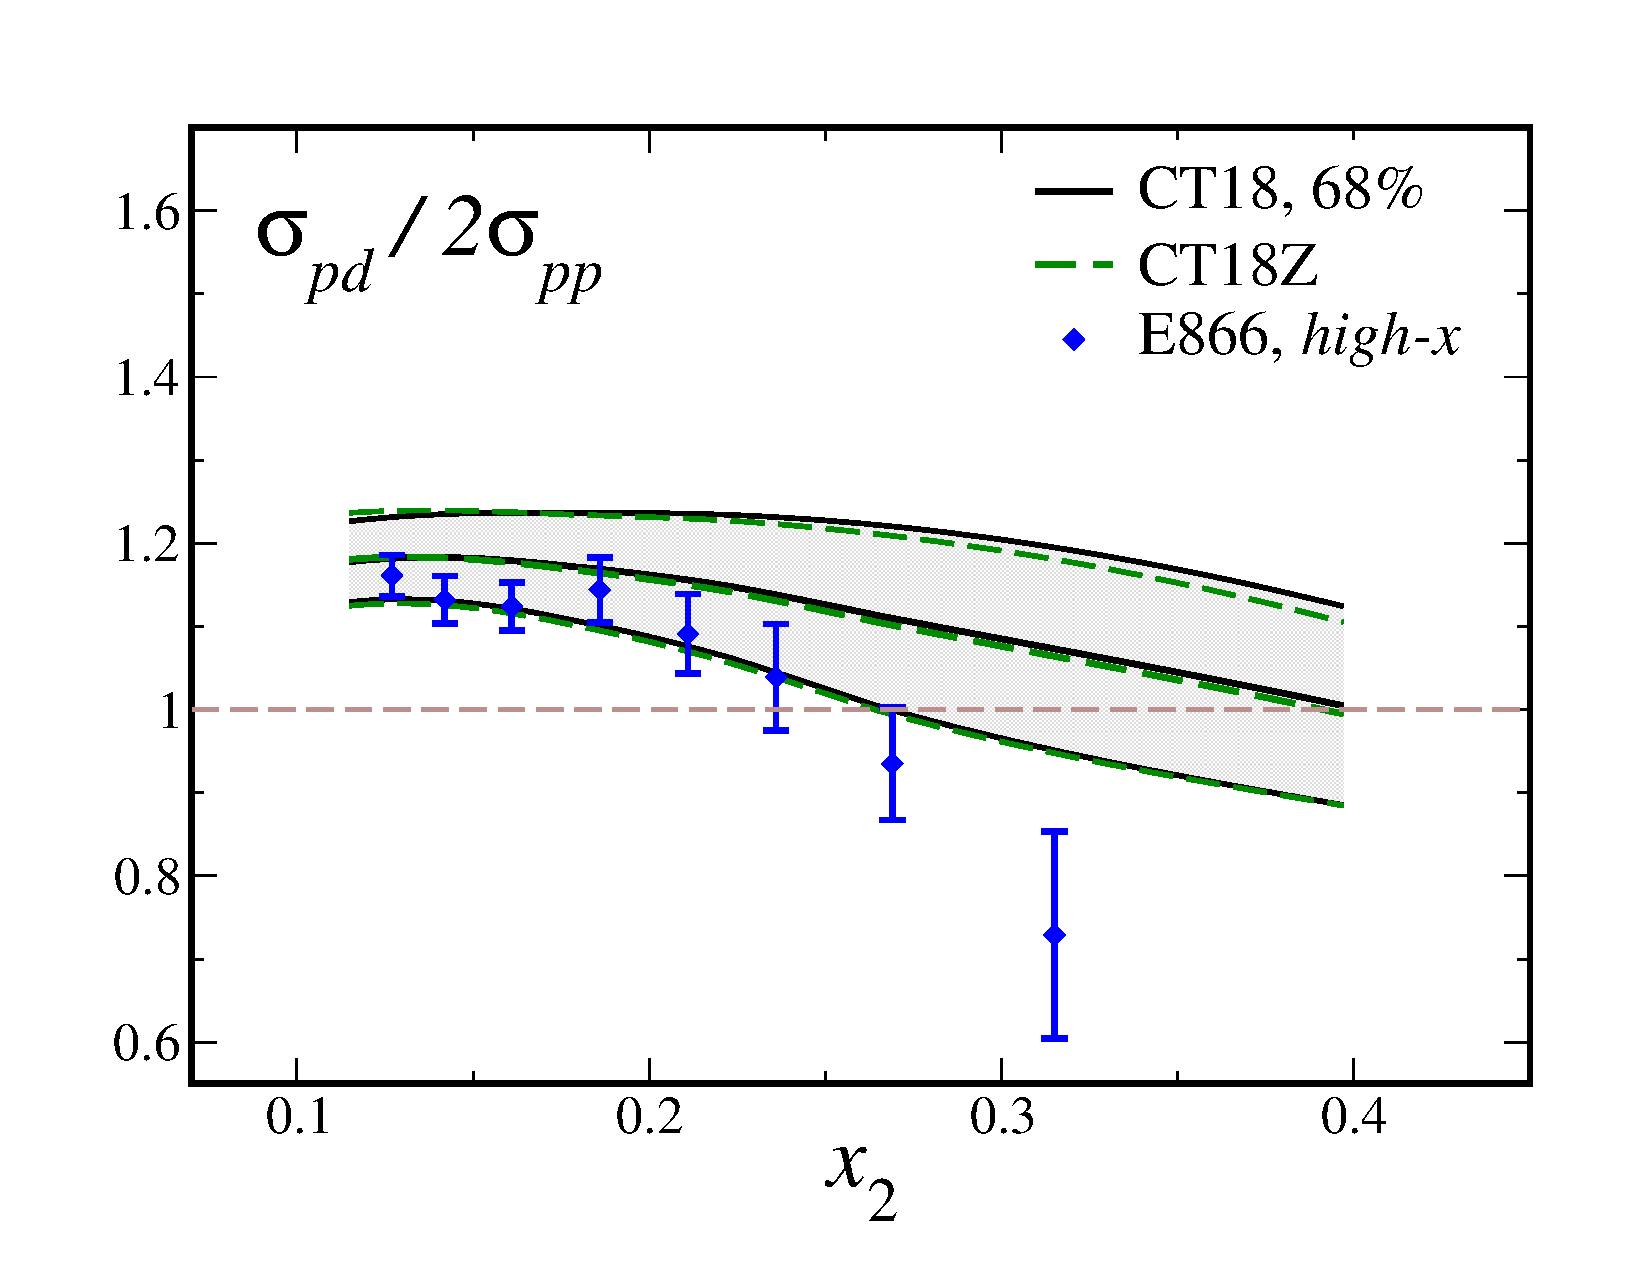
\includegraphics[width=0.75\textwidth]{./fig/CT18-prediction_E866_68.pdf}
	\end{center}
	\vspace{-2ex}
	\caption{ Theoretical predictions based on CT18 (black outer band) and CT18Z (Green inner band) for the fixed-target Drell-Yan
	cross section, $\sigma_{pd} \big/ 2\sigma_{pp}$, in the region of larger $x_2 \gtrsim 0.1$ to be probed by the SeaQuest experiment \cite{Aidala:2017ofy} at Fermilab. For comparison, we also plot the higher-$x_2$ portion of the older E866 data \cite{Towell:2001nh} (blue diamonds). }
\label{fig:hix_DY}
\end{figure}

Intriguingly, E866 \cite{Towell:2001nh} found evidence that the cross section ratio dropped below unity, $\sigma_{pd} \big/ 2\sigma_{pp} < 1$,
as $x_2$ approached and exceeded $x \gtrsim 0.25$, as seen by the higher $x_2$ portion of the E866 ratio points shown
in Fig.~\ref{fig:hix_DY}. This fact was surprising on the grounds of a number of theoretical models.
%
%
The E866 results therefore stimulated an interest in performing a similar measurement out to larger $x_2$ with higher
precision --- the main objective of the subsequent SeaQuest/E906 experiment at Fermilab \cite{Aidala:2017ofy} from which
results are expected soon. For this reason, we illustrate in Fig.~\ref{fig:hix_DY} theoretical predictions based upon our
updated CT18 (black band) and CT18Z (green band) global analyses at the 68\% C.L.~to higher $x_2$ beyond that probed by E866.  While CT18
and CT18Z are constrained to the E866 ratio data, the theoretical prediction for
the deuteron-to-proton ratio remains above or consistent with unity out to
$x\! <\! 0.4$.  More precision data in the high-$x$ region will be instrumental in
resolving the behavior of the cross-section ratio and its implications for the
nucleon sea.
 
\clearpage
